\documentclass[a4paper,10pt]{report}
\usepackage[utf8]{inputenc}
\usepackage{amssymb}
\usepackage{amsthm}
\usepackage{amsmath}
\usepackage{graphicx}
\usepackage{steinmetz}
\usepackage{booktabs}
\usepackage[mathscr]{euscript}
\usepackage[bookmarksopen, linktocpage]{hyperref}
\setlength{\parindent}{0pt}

\newcommand{\norm}[1]{\lVert#1\rVert} 		%Double vertical bars for norms
\newcommand{\ip}[2]{\langle#1,#2\rangle}	%Inner product
\newcommand{\vb}[1]{\mathbf{#1}}		%Bold vector

\makeatletter
\renewcommand*\env@matrix[1][*\c@MaxMatrixCols c]{%
  \hskip -\arraycolsep
  \let\@ifnextchar\new@ifnextchar
  \array{#1}}
\makeatother
% Augmented matrices. Use like this:
% \begin{pmatrix}[cc|c]

\begin{document}
\title{Circuits, Spring 2014 Notes}
\author{Zack Garza}
\maketitle
\tableofcontents

\chapter{LRC}
\section{Inductors}
Current can not change instantaneously.
Can be combined like resistors.
Behaves like a short if current is constant.

\begin{figure}[htpb]
	\begin{centering}
	\begin{center}
	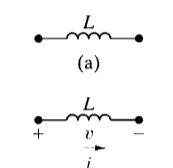
\includegraphics{./inductor_sign_convention.png}
	\caption{Inductor Sign Conventions}
	\label{fig:inductor_sign_convention}
	\end{center}
	\par\end{centering}
\end{figure}

\begin{align*}
	v 		&= L \frac{di}{dt} \\
	i{t} 	&= \frac{1}{L} \int_0^t v dt + i(t_0) \\
	p 		&= Li\frac{di}{dt} \\
	w 		&= \frac{1}{2}Li^2
\end{align*}

Mutual Inductance
\begin{align*}
	v_1 = L_1\frac{di_1}{dt} + M_{12}\frac{di_2}{dt} \\
	v_2 = L_2\frac{di_2}{dt} + M_{21}\frac{di_1}{dt} \\
	M = k\sqrt{L_1L_2} \\
	L = N^2\mathcal{P}
\end{align*}
$M_2$ = $M_1$ if coils are not magnetic.
$N$ is the number of turns in an inductor, and $\mathcal{P}$ is the permeance of the space. For nonmagnetic materials, the permeances are equal.

Energy stored in coupled coils:
\begin{align*}
	w = \frac{1}{2}L_1i_1^2 + \frac{1}{2}L_2i_2^2 \pm Mi_1i_2
\end{align*}

\textit{Notes to self:}
Should really review the dot convention.
Review equivalence reductions - know how to collapse triangles!


\section{Capacitors}
Voltage can not change instantaneously.
Behaves like an open circuit if voltage is constant.
\begin{figure}[htpb]
	\begin{centering}
	\begin{center}
	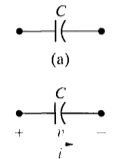
\includegraphics{./capacitor_sign_convention.png}
	\caption{Capacitor Sign Conventions}
	\label{fig:capacitor_sign_convention}
	\end{center}
	\par\end{centering}
\end{figure}

\begin{align*}
	i &= C\frac{dv}{dt} \\
	v(t) &= \frac{1}{C}\int_{t_0}^t i dt + v(t_0) \\
	p &= Cv\frac{dv}{dt} \\
	w &= \frac{1}{2}Cv^2
\end{align*}


\chapter{7 - LRC Response}
Review:
Voltage Divider:
\begin{align*}
	V_{R2} &= V_s\frac{R_2}{R_1 + R_2}\\
	V_{R2} &= V_s\frac{R_2 || R_L}{R_1 + (R_2 || R_L)}
\end{align*}
\begin{figure}[!h]
	\begin{centering}
	\begin{center}
	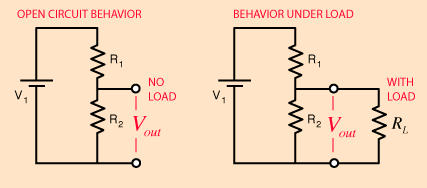
\includegraphics[width=\linewidth]{./voltage_divider.png}
	\caption{Voltage Divider}
	\label{fig:voltage_divider}
	\end{center}
	\par\end{centering}
\end{figure}

Current Divider:
\begin{figure}[!H]
	\begin{centering}
	\begin{center}
	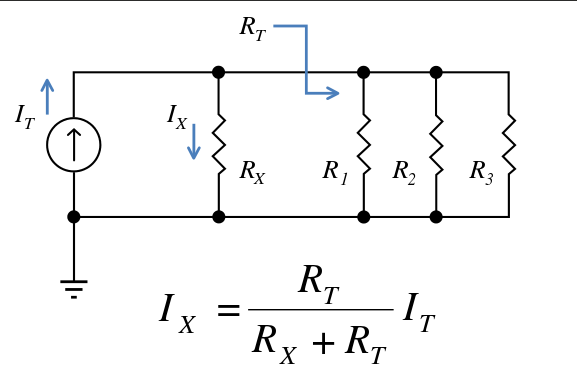
\includegraphics[width=\linewidth]{./current_divider.png}
	\caption{Current Divider}
	\label{fig:current_divider}
	\end{center}
	\par\end{centering}
\end{figure}

RL
\begin{align*}
i(t) = i_0\mathrm{e}^{-(L/R)t}
\end{align*}
Inductors force current in a branch to not change instantaneously.
%TODO: Needs serious update!

\chapter{Sinusoidal Steady-State Analysis}
The general expression for a sinusoidally varying signal is generally written as
\begin{align*}
	v(t) = V_m \cos(\omega t + \phi) \\
	i(t) = I_m \cos(\omega t + \phi)
\end{align*}
where the frequency $\omega$ of the response will be the same as that of the source, provided all circuit elements are linear. %?

In review, there are a few handy relationships to know.
\begin{align*}
	&f=\frac{1}{T} &\omega = 2\pi f = \frac{2\pi}{T} \text{(rad/s)}
\end{align*}
where it is common to express the phase angle $\phi$ and the quantity $\omega t$ in radians.

It is also convenient to define the \textbf{rms} voltage, which is the square root of the mean value of the squared function. This is obtained by squaring the function and finding the average value over one period, and is given by
\begin{align*}
	V_{\text{rms}} = \sqrt{\frac{1}{T}\int_{t_0}^{t_0 + T} V_m^2 \cos^2(\omega t + \phi)dt} = \frac{V_m}{\sqrt{2}},
\end{align*}
which depends only on the maximum voltage.

A few trig identities also come in handy when working with sinusoids.
\begin{align*}
	\sin(\theta) = \cos(\theta-\pi) \\
	\cos(\alpha-\beta) = \cos\alpha\cos\beta + \sin\alpha\sin\beta
\end{align*}

Given an RL circuit, applying Kirchhoff's Voltage Law yields the ODE
\begin{align*}
	L\frac{di}{dt} + Ri = V_m\cos(\omega t + \phi)
\end{align*}

Solving for $i$, skipping the work, yields
\begin{align*}
	i(t) = \frac{-V_m}{\sqrt{R^2 +\omega^2 L^2}}\cos(\phi - \theta)e^{-(R/L)t}
	+ \frac{V_m}{\sqrt{R^2 + \omega^2 L^2}}\cos(\omega t + \phi - \theta) \\
	\text{where } \tan\theta = \frac{\omega L}{R}
\end{align*}
which shows that the total response is the sum of a transient and a steady-state component.

For this analysis, we are only interested in obtaining the steady-state response. This reduces the problem from an ODE to simply finding the maximum amplitude and the phase angle of the response, since the waveform and frequency are already known to match the source.

It turns out that the analysis is much easier in the frequency domain, and it is convenient to use phasors to find these quantities. Recalling Euler's identity,
\begin{align*}
	e^{\pm j\theta} = \cos\theta \pm j\sin\theta \\
	\text {where } \\
	\cos\theta = \Re\left\{e^{j\theta}\right\} \\
	\sin\theta = \Im\left\{e^{j\theta}\right\}
\end{align*}

We can then define the phasor transform $\mathcal{P}$ such that
\begin{align*}
	\mathcal{P}\left\{ V_m\cos(\omega t 	+ \phi) 	\right\}
	&= V_m \Re \left\{ e^	{j(\omega t 	+ \phi)}	\right\} \\
	&= V_m \Re \left\{ e^	{j\omega t}   e^{j\phi}		\right\} \\
	&= 	   \Re \left\{ V_m e^	{j\omega t}   e^{j\phi}		\right\} \\
	&= V_m e^{j\phi} = \vb{V} ~(=V_m\phase{\phi}.
\end{align*}
where $\vb{V}$ carries information about the amplitude and phase angle of the sinusoid. This takes a sinusoid to its polar form in the complex plane, or in other words, moves from the time domain to the frequency domain.

The inverse phasor transform is similarly defined as
\begin{align*}
	\mathcal{P}^{-1}\left\{ V_m e^{j\phi}\right\} = \Re\left\{ V_m e^{j\phi}e^{j\omega t} \right\},
\end{align*}
which moves from the frequency domain to the time domain.

The phasor can also be written in rectangular form as
\begin{align*}
	\vb{V} = V_m \cos\phi + jV_m\sin\phi.
\end{align*}

$V/i$ relationships in the frequency domain are generally of the form $\vb{V} = Z\vb{I}$, where $Z$ is defined to be the \textbf{impedance} of the element. This is algebraically similar to Ohm's Law, using algebra of complex numbers.

Impedance in the frequency domain is analogous to resistance, inductance, or capacitance in the time domain. The imaginary part of the impedance of called \textbf{reactance}.

\begin{table}[h]
\centering{}
\begin{tabular}{@{}lll@{}}
\toprule
\textbf{Element} 	&\textbf{Impedance} 		&\textbf{Reactance} \\ \midrule
Resistor			&$R$ 						&-- 				\\
Inductor			&$j\omega L$				&$\omega L$ 		\\
Capacitor			&$j(-1/\omega C)$  			&$-1/\omega C$ 		\\ \bottomrule
\end{tabular}
\end{table}


Most familiar laws hold in the frequency domain. Kirchhoff's Laws can be written in terms of phasor voltages as
\begin{align*}
	&\sum_{i=1}^n \vb{V}_i = 0 &(\text{KVL}) \\
	&\sum_{i=1}^n \vb{I}_i = 0 &(\text{KCL})
\end{align*}
In terms of series/parallel combinations, impedances can be combined in the same manner that resistances are combined. For this reason, it is common to rewrite impedances in units of $\omega$ as a mnemonic.

When combining equivalent elements, it is useful to define the \textbf{admittance} $Y = \frac{1}{Z} = G + jB$, where the real number $G$ is referred to as \textbf{conductance} and the complex number $B$ is the \textbf{susceptance}. This allows parallel elements to be simplified as $Y_{\text{eq}} = \sum_{i=0}^n Y_i$, and changes it $V/i$ relationship to $\vb{V} = \vb{I}/Y$.

\begin{table}[h]
\centering{}
\begin{tabular}{@{}lll@{}}
\toprule
\textbf{Element} 	&\textbf{Admittance ($Y$)} 	&\textbf{Susceptance} 	\\ \midrule
Resistor			&$G$ (conductance) 			&-- 					\\
Inductor			&$j(-1/\omega L)$			&$-1/\omega L$ 			\\
Capacitor			&$j\omega C$  				&$\omega C$ 			\\ \bottomrule
\end{tabular}
\end{table}

Similarly, $\Delta-Y$ transformations can be applied in exactly the same way, as can Northon/Thevenin equivalent sources, the Node Voltage Method, and the Mesh-Current Method.

\hrulefill
\center{
A handy note to remember:

In an inductor, voltage leads current by $90^{\circ}$.

In a capacitor, current leads voltage by $90^{\circ}$.}

\hrulefill





\end{document}